\documentclass[10pt,a4paper,spanish]{report}

\usepackage[spanish]{babel}
\usepackage[utf8]{inputenc}
\usepackage{amsmath, amsthm}
\usepackage{amsfonts, amssymb, latexsym}
\usepackage{enumerate}
\usepackage[official]{eurosym}
\usepackage{graphicx}
\usepackage[usenames, dvipsnames]{color}
\usepackage{colortbl}
\usepackage{multirow}
\usepackage{fancyhdr}
\usepackage[all]{xy}
\usepackage{minted}
\usepackage{tikz}
\usepackage{pgfplots}
\usepackage{algpseudocode}
\usepackage{listings}
\usepackage{titlesec}

\pgfplotsset{compat=1.5}

% a4large.sty -- fill an A4 (210mm x 297mm) page
% Note: 1 inch = 25.4 mm = 72.27 pt
%       1 pt = 3.5 mm (approx)

% vertical page layout -- one inch margin top and bottom
\topmargin      0 mm    % top margin less 1 inch
\headheight     0 mm    % height of box containing the head
\headsep       10 mm    % space between the head and the body of the page
\textheight   250 mm
\footskip      14 mm    % distance from bottom of body to bottom of foot

% horizontal page layout -- one inch margin each side
%\oddsidemargin    0   mm    % inner margin less one inch on odd pages
%\evensidemargin   0   mm    % inner margin less one inch on even pages
%\textwidth      159.2 mm    % normal width of text on page

\usepackage[math]{iwona}
\usepackage[T1]{fontenc}
\usepackage{inconsolata}

\usepackage[pdftex, bookmarks=true,
	bookmarksnumbered=false, % true means bookmarks in
	% left window are numbered
	bookmarksopen=false,     % true means only level 1
	% are displayed.
	colorlinks=true,
linkcolor=webblue]{hyperref}

\definecolor{webgreen}{rgb}{0, 0.5, 0} % less intense green
\definecolor{webblue}{rgb}{0, 0, 0.5}  % less intense blue
\definecolor{webred}{rgb}{0.5, 0, 0}   % less intense red
\definecolor{dblackcolor}{rgb}{0.0,0.0,0.0}
\definecolor{dbluecolor}{rgb}{.01,.02,0.7}
\definecolor{dredcolor}{rgb}{0.8,0,0}
\definecolor{dgraycolor}{rgb}{0.30,0.3,0.30}

\newcommand{\HRule}{\rule{\linewidth}{0.5mm}} % regla horizontal para  el titulo

\pagestyle{fancy}
%con esto nos aseguramos de que las cabeceras de capítulo y de sección vayan en minúsculas

\renewcommand{\chaptermark}[1]{%
	\markboth{#1}{}}
\renewcommand{\sectionmark}[1]{%
	\markright{\thesection\ #1}}
\fancyhf{} %borra cabecera y pie actuales
\fancyhead[LE,RO]{\bfseries\thepage}
\fancyhead[LO]{\bfseries\leftmark}
\renewcommand{\headrulewidth}{0.5pt}
\renewcommand{\footrulewidth}{0pt}
\addtolength{\headheight}{0.5pt} %espacio para la raya
\fancypagestyle{plain}{%
	\fancyhead{} %elimina cabeceras en páginas "plain"
	\renewcommand{\headrulewidth}{0pt} %así como la raya
}

%%%%% Para cambiar el tipo de letra en el título de la sección %%%%%%%%%%%
\chapterfont{\fontfamily{pag}\selectfont} %% for chapter if you want
\sectionfont{\fontfamily{pag}\selectfont}
\subsectionfont{\fontfamily{pag}\selectfont}
\subsubsectionfont{\fontfamily{pag}\selectfont}
\titleformat{\chapter}{\normalfont\Huge}{}{0pt}{\Huge} % Capítulos sin "Capítulo x" encima del título

\renewcommand{\labelenumi}{\arabic{enumi}. }
\renewcommand{\labelenumii}{\labelenumi\alph{enumii}) }
\renewcommand{\labelenumiii}{\labelenumii\roman{enumiii}: }

\newmintedfile[myCpp]{cpp}{
	linenos,
	numbersep=5pt,
	gobble=0,
	frame=lines,
	framesep=2mm,
	fontsize=\footnotesize
}

\newmintedfile[myLex]{bash}{
	linenos,
	numbersep=5pt,
	gobble=0,
	frame=lines,
	framesep=2mm,
	breaklines=true,
	fontsize=\footnotesize
}

\newmintedfile[myLatex]{tex}{
	linenos,
	numbersep=5pt,
	gobble=0,
	frame=lines,
	framesep=2mm,
	tabsize=3,
}

\newmintedfile[myHtml]{html}{
	linenos,
	numbersep=5pt,
	gobble=0,
	frame=lines,
	framesep=2mm,
	tabsize=3,
}

\title{Modelos de Computación}
\author{David Sánchez Jiménez}

\begin{document}
\begin{titlepage}
	\begin{center}
		\HRule \\[0.8cm]
		\textsc{\huge Modelos de\\[0.5cm] Computación}\\[1.6cm]
		\HRule \\[1cm]
		\begin{flushleft}
			\emph{Hecho por:}\\
			David Sánchez Jiménez
		\end{flushleft}
		\vspace{12cm}
		\large{\today}\\
		\vspace{0.5cm}
		\htmladdnormallink{
\includegraphics[width=2cm]{88x31.png}}
		{http://creativecommons.org/licenses/by-nc/4.0/}\\[0.5cm]
		\texttt{Prácticas de Modelos de Computación\\ by
			\href{mailto:dasaji92@gmail.com}{David Sánchez Jiménez} is licensed under a \htmladdnormallink{Creative Commons Reconocimiento-NoComercial-CompartirIgual 4.0 Internacional License}
			{http://creativecommons.org/licenses/by-nc/4.0/}}.\\[3mm]
	\end{center}
\end{titlepage}

\tableofcontents
\newpage

%%%%%%%%%%%%%%%%%%%%%%%%%%%%%%% Ejercicio  1 %%%%%%%%%%%%%%%%%%%%%%%%%%%%%%%%%%%%%

\chapter{Ejercicio 1}
\section{Enunciado:}

\noindent
Sea la gramática $G = (V,T,P,S)$, donde $V = \{S,A,B\}$,$T=\{a,b\}$, el símbolo de partida es $S$ y las reglas, $P$, son:
\begin{displaymath}
	S \rightarrow aB, \qquad\ S \rightarrow bA, \qquad\ A \rightarrow a, \qquad\ A \rightarrow aS,
\end{displaymath}
\begin{displaymath}
	A \rightarrow bAA, \qquad\ B \rightarrow b, \qquad\ B \rightarrow bS, \qquad\ B \rightarrow aBB
\end{displaymath}

\noindent
Demostrar que esta gramática genera el lenguaje
\begin{displaymath}
	L(G) = \{u~ | ~u \in \{a,b\}^+ ~y~ N_a(u) = N_b(u) \}
\end{displaymath}

\noindent
donde $N_a(u)$ y $N_b(u)$ son el número de apariciones de símbolos $a$ y $b$, en $u$, respectivamente y $\{a,b\}^+$ representa todas las cadenas existentes combinando $a$ y $b$ en cualquier orden excluyendo la cadena vacía ($\varepsilon$).

\section{Solución:}

\noindent
Las reglas de producción de esta gramática generan un lenguaje con el mismo número de símbolos terminales $a$ y $b$. A partir del símbolo inicial $S$ podemos generar $aB$ o $bA$. Vamos a intentar generar una cadena que no cumpla esta condición, como por ejemplo la cadena $aaabb$, para ello seguimos los siguientes pasos:

\begin{displaymath}
	S \rightarrow aB \rightarrow aaBB \rightarrow aaaBBB \rightarrow aaabBB \rightarrow aaabbB
\end{displaymath}

\noindent
Ya hemos conseguido la cadena $aaabb$ pero aún nos queda una variable $B$ y no tenemos ninguna regla de producción para cambiarla por $\varepsilon$ así que nos vemos forzados a cambiar dicha $B$ por otra $b$, por $bS$ o por $aBB$.

\noindent
Ahora vamos a intentar generar la palabra $bbbaa$, para ello seguimos los siguientes pasos:

\begin{displaymath}
	S \rightarrow bA \rightarrow bbAA \rightarrow bbbAAA \rightarrow bbbaAA \rightarrow bbbaaA.
\end{displaymath}

\noindent
Ya hemos conseguido la cadena $bbbaa$ pero aún nos queda una variable $A$ y no tenemos ninguna regla de producción para cambiarla por $\varepsilon$ así que nos vemos forzados a cambiar dicha $A$ por otra $a$, por $aS$ o por $bAA$. \\

\noindent
Con esto demostramos que a partir del símbolo inicial $S$ cojamos el camino que cojamos a la fuerza esta gramática genera palabras con el mismo número de simbolos terminales $a$ y $b$ por lo que se cumple la propiedad $N_a(u) = N_b(u)$.

%%%%%%%%%%%%%%%%%%%%%%%%%%%%%%% Ejercicio  2 %%%%%%%%%%%%%%%%%%%%%%%%%%%%%%%%%%%%%

\chapter{Ejercicio 2}
\section{Enunciado:}

\noindent
Determinar si la gramática $G = (\{S,A,B\}, \{a,b,c,d\}, P, S)$ genera un lenguaje de tipo 3 donde P es el conjunto de reglas de producción:
\begin{displaymath}
	S \rightarrow AB, \qquad\ A \rightarrow Ab \qquad\ A \rightarrow a
\end{displaymath}
\begin{displaymath}
	B \rightarrow cB \qquad\ B \rightarrow d
\end{displaymath}

\section{Solución:}

\noindent
Debemos comprobar las reglas de producción de esta gramática generan palabras que no pertenecen al lenguaje $L(G) = \{ab^ic^jd : i,j \epsilon \mathbb{N}\}$. A partir de las reglas de producción podemos observar que $A$ genera subcadenas que empiezan por $'a'$ seguidas de un número $i$ de $'b'$ y que $B$ genera subcadenas que empiezan por un número $j$ de $'c'$ y acaban en $'d'$. \\

\noindent
También podemos observar que es una gramática libre de contexto de tipo 2 ya que todas sus producciones son de de la forma ''variable-terminal'', ''terminal-variable'' o ''variable-variable''. \\

\noindent
Ahora debemos estudiar si podemos conseguir que genere un lenguaje regular con las reglas de producción de las que disponemos, las cuales deben ser de la forma $A \rightarrow uB$ o $A \rightarrow B$ segun la Jerarquía de Chomsky. Para ello vamos a utilizar las siguientes reglas de producción:

\begin{displaymath}
	S \rightarrow aB \qquad B \rightarrow bB \qquad B \rightarrow C
\end{displaymath}
\begin{displaymath}
	C \rightarrow cC \qquad C \rightarrow d
\end{displaymath}

\noindent
Con la regla $S \rightarrow aB$ generamos la primera $'a'$ seguida de la variable $'B'$, la cual sustituiremos mediante la regla $B \rightarrow bB$ para conseguir generar un número $i$ de $'b'$ deseado. Una vez tengamos todas las $'b'$ que queramos podemos pasar a $'C'$ mediante la regla $B \rightarrow C$ a partir de la cual podremos generar un número $j$ de $'c'$ con la regla $C \rightarrow cC$. Para finalizar el proceso cambiamos una variable $'C'$ por una $'d'$, siendo este el último simbolo con el cual formaremos nuestra palabra. \\

\noindent
Con esto, demostramos que con estas reglas de producción de tipo 3, nos encontramos con una gramática regular que genera el mismo lenguaje que podiamos obtener mediante las reglas de producción iniciales, por lo que demostramos que esta gramática es de tipo tres y por tanto este lenguaje tambien lo es.

%%%%%%%%%%%%%%%%%%%%%%%%%%%%%%% Ejercicio 3 %%%%%%%%%%%%%%%%%%%%%%%%%%%%%%%%%%%%%

\chapter{Ejercicio 3}

\section{Enunciado:}

\noindent
Crear un autómata que dada la entrada 1100111 genere la salida 1000101.

\section{Solución:}
\noindent
Debemos implementar un decodificador de tipo Mealy del que conocemos la entrada, que es 1100111 y el valor de salida que debemos obtener es 1000101. Este valor lo obtenemos de los siguientes datos:

\begin{itemize}
	\item Si es el primer símblolo escrito: $0 \rightarrow 0$ y $1 \rightarrow 1$.
	\item Si no es el primer simbolo escrito:
	      \begin{itemize}
	      	\item Si el anterior simbolo escrito es un 0: $0 \rightarrow 0$ y $1 \rightarrow 1$.
	      	\item Si el anterior simbolo escrito es un 1: $0 \rightarrow 1$ y $1 \rightarrow 0$.
	      \end{itemize}
\end{itemize}

\noindent
Para implementar la máquina de Mealy, conocemos el valor de entrada y el valor de salida que queremos obtener y cuya salida está asociada a la transición de estados entre $q_0$ y $q_1$.

\begin{itemize}
	\item $q_0$: En este estado, el símbolo anterior escrito tiene que ser el símbolo inicial escrito o un 0, por lo que será el estado inicial. Cuando tengamos un 0 en el estado $q_0$ la salida que obtendremos será 0 y no habrá ninguna transición ya que $q_0$ tomará el símbolo anterior escrito como un 0. Si fuese un 1, se pasaría a $q_1$, ya que el símbolo anterior escrito debe ser un 1 y por tanto, la salida obtenida será un 1.
	\item $q_1$: En este estado, el símbolo anterior escrito es un 1, por lo que en caso de que llegase un 0, la salida será un 1 y no habrá transición, de tal forma que si llega un 1, la salida obtenida será un 0 y se pasará al estado $q_0$.
\end{itemize}

\begin{figure}[!hbp]
	\centering  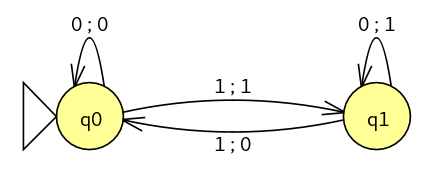
\includegraphics[width=0.8\textwidth]{Imagenes/Ejercicio3-1.png}
\end{figure}

\newpage
\noindent
Vamos a probar con JFLAP nuestro decodificador para ver si es correcto:

\begin{figure}[!hbp]
	\centering  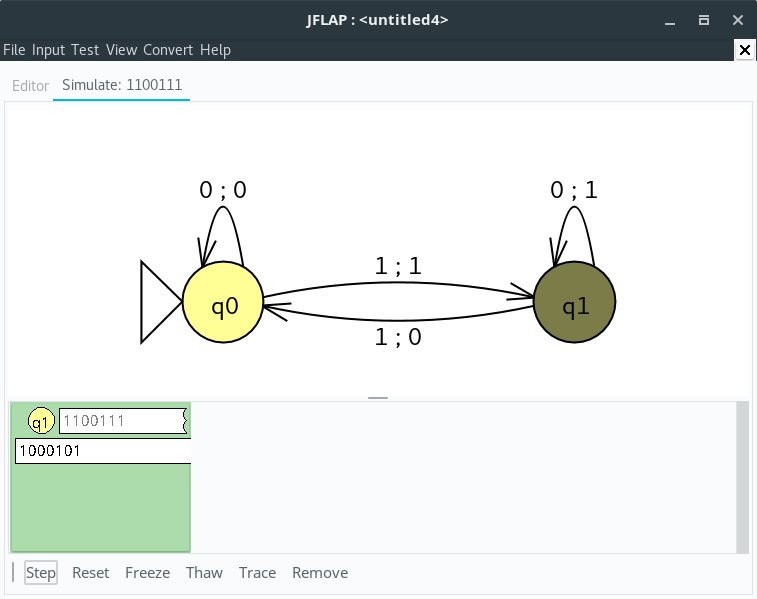
\includegraphics[width=0.8\textwidth]{Imagenes/Ejercicio3-2.png}
\end{figure}

\noindent
Con esto comprobamos que al introducirle como entrada 1100111 obtenemos como salida 1000101.

%%%%%%%%%%%%%%%%%%%%%%%%%%%%%%% Ejercicio  4 %%%%%%%%%%%%%%%%%%%%%%%%%%%%%%%%%%%%%

\chapter{Ejercicio 4}

\section{Enunciado:}

\noindent
Compilar el siguiente fichero lex el cual reconoce números enteros y reales y hacer varias pruebas con el.

\myLex[label={ejemplo.l}]{Lex/ejemplo/ejemplo.l}

\newpage
\section{Solución:}

\subsection{Ejecución del fichero LeX de ejemplo}

\noindent
Disponemos de el fichero .lex con el ejemplo que viene en las transparencias de clase y un archivo de entrada para probar nuestro programa.
En las siguientes capturas de pantalla documentaré el proceso a seguir para conseguir ejecutar el ejemplo. \\

\noindent
Primero debemos convertir el .lex en un fichero .c para poder compilarlo.

\begin{figure}[!hbp]
	\centering  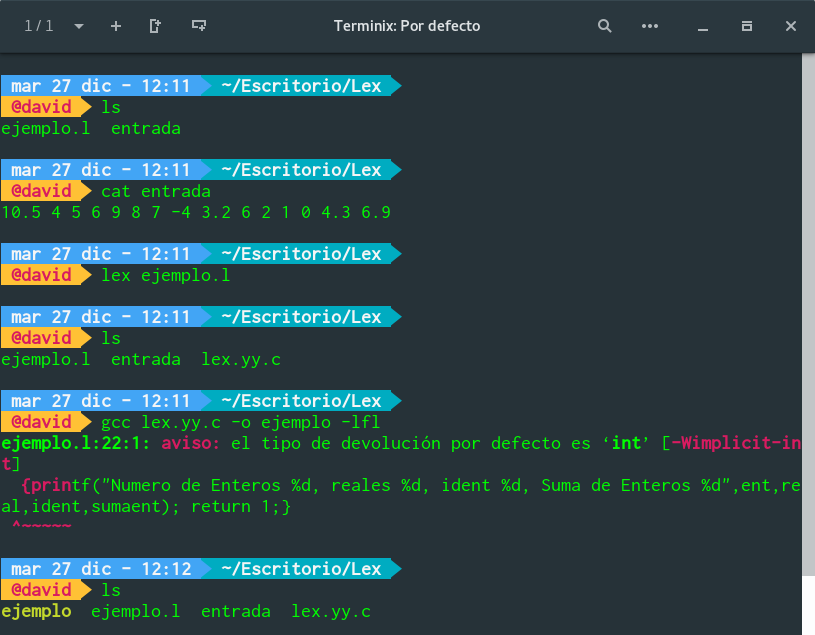
\includegraphics[width=0.85\textwidth]{Imagenes/Ejercicio4-1.png}
\end{figure}

\noindent
Una vez compilado ya podemos ejecutarlo. Le paso un archivo de entrada el cual contiene números para probar el correcto funcionamiento del programa.

\begin{figure}[!hbp]
	\centering  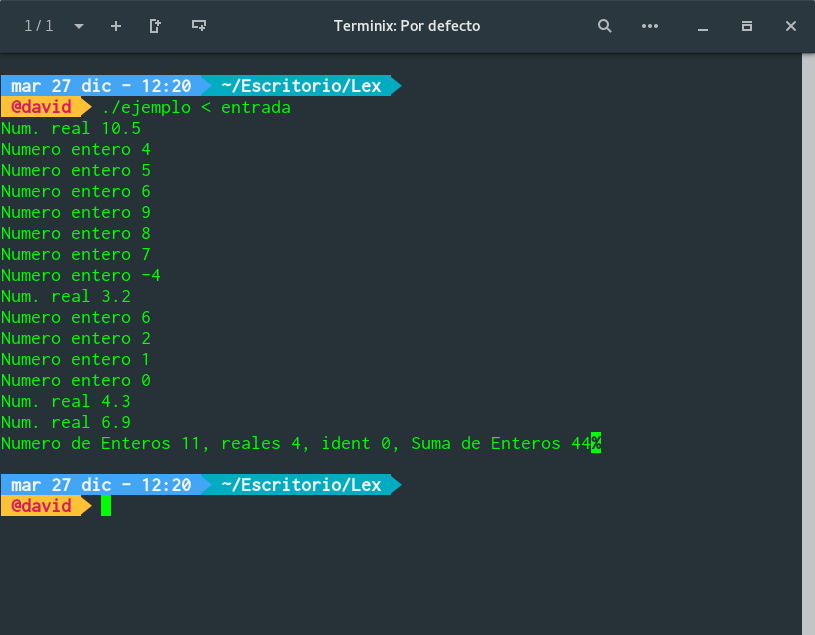
\includegraphics[width=0.85\textwidth]{Imagenes/Ejercicio4-2.png}
\end{figure}

\newpage
\subsection{Creación de mi fichero LEX:}

\noindent
Como ampliación de esta práctica he realizado un conversor de HTML a Latex. Para probarlo he creado un archivo llamado test.html el cual contiene distintos elementos básicos de HTML los cuales vamos a convertir a LaTeX. Tras la ejecución del programa, se generará un archivo llamado salida.tex que contiene los distintos elementos del archivo de entrada listo para su compilación en PDF. \\

\noindent
A continuación adjunto una captura de pantalla de la compilación y ejecución así como el código del programa y los ficheros de entrada y salida que he utilizado para su ejecución.

\begin{figure}[!hbp]
	\centering  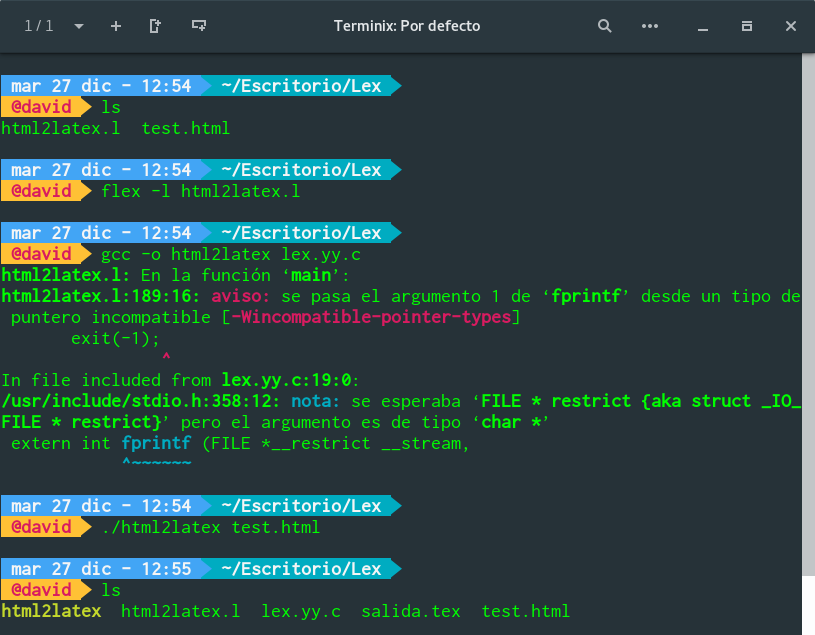
\includegraphics[width=0.85\textwidth]{Imagenes/Ejercicio4-3.png}
\end{figure}

\newpage
\myLex[label={html2latex.l}]{./Lex/html2latex/html2latex.l}

\newpage
\myHtml[label={test.html}]{./Lex/html2latex/test.html}

\newpage
\myLatex[label={salida.tex}]{./Lex/html2latex/salida.tex}

%%%%%%%%%%%%%%%%%%%%%%%%%%%%%%% Ejercicio  5 %%%%%%%%%%%%%%%%%%%%%%%%%%%%%%%%%%%%%

\chapter{Ejercicio 5}

\section{Enunciado:}

\noindent
Dada la siguiente gramática, demostrar que el lenguaje que genera no es inminentemente ambiguo.

\begin{displaymath}
	E \rightarrow I, \qquad\ E \rightarrow I-E \qquad\ E \rightarrow E-I \qquad I \rightarrow a | b | c | d
\end{displaymath}

\section{Solución:}

\noindent
Para comprobar si la gramática es ambigua vamos a comprobar si existe una palabra la cual tenga dos árboles de derivación distintos. Para ello utilizaremos la palabra abcd:

\begin{figure}[!hbp]
	\centering  \includegraphics[width=0.85\textwidth]{Imagenes/Ejercicio5.png}
\end{figure}

\noindent
Por lo que demostramos que la palabra abcd se puede generar con las siguientes derivaciones:

\begin{enumerate}
	\item $E \Rightarrow I-E \Rightarrow a-E \Rightarrow a-I-E \Rightarrow a-b-E \Rightarrow a-b-I-E \Rightarrow$ \\ $		\Rightarrow a-b-c-E \Rightarrow a-b-c-I \Rightarrow a-b-c-d$

	\item $E \Rightarrow E-I \Rightarrow E-d \Rightarrow E-I-d \Rightarrow E-c-d	\Rightarrow E-I-c-d \Rightarrow$ \\$\Rightarrow E-b-c-d \Rightarrow I-b-c-d \Rightarrow a-b-c-d$
\end{enumerate}

\noindent
Para conseguir que el lenguaje generado no sea ambiguo podemos eliminar la regla $E \rightarrow I-E$ o la regla $E \rightarrow E-I$.

%%%%%%%%%%%%%%%%%%%%%%%%%%%%%%% Ejercicio  6 %%%%%%%%%%%%%%%%%%%%%%%%%%%%%%%%%%%%%

\chapter{Ejercicio 6}

\section{Enunciado:}

\noindent
Dada la siguiente gramática libre de contexto:

\begin{displaymath}
	S \rightarrow A | BCa | aDcd | EDF \qquad A \rightarrow aAb | c \qquad B \rightarrow CD | ECd | Ad | \varepsilon
\end{displaymath}
\begin{displaymath}
	C \rightarrow Cc | Bb | AaE | c \qquad D \rightarrow aDd | Dd | \varepsilon \qquad E \rightarrow aaEB | EFG
\end{displaymath}


\begin{enumerate}
	\item Elimina las producciones inutiles.
	\item Elimina las producciones nulas.
	\item Elimina las producciones unitarias.
	\item Pasa a forma normal de Chomsky.
	\item Pasa a forma normal de Greibach.
\end{enumerate}

\section{Solución:}

\noindent
Para la realización de este ejercicio he realizado adicionalmente los pasos con la herramienta JFLAP para la corrección de los posibles fallos durante el proceso.

\begin{enumerate}
	\item Eliminación de las producciones nulas.

	      \noindent
	      Primero debemos identificar todas las producciones nulas las cuales son $B \rightarrow \varepsilon$ y $D \rightarrow \varepsilon$. \\

	      \noindent
	      A continuación, para cada producción que en su parte derecha tuviese como mínimo una de las producciones identificadas en el paso anterior, tenemos que añadir todas las producciones que podriamos conseguir usando la produccion que deseamos eliminar. \\

	      \noindent
	      Por ultimo, debemos eliminar dichas producciones, por lo que nos quedamos con lo siguiente: \\

	      $S \rightarrow A | BCa | aDcd | EDF | Ca | acd | EF$ \\
	      $A \rightarrow aAb | c$ \\
	      $B \rightarrow CD | Ad | ECd | C$ \\
	      $C \rightarrow Cc | Bb | AaE | c | b$ \\
	      $D \rightarrow aDd | Dd | ad | d$ \\
	      $E \rightarrow aaEB | EFG | aaE $

	      \newpage
	\item Eliminación de las producciones unitarias.

	      \noindent
	      Ahora debemos eliminar las producciones unitarias, las cuales son $H = \{A, C\}$, y añadir a las producciones que se podían obtener a partir de las producciones eliminadas. Tras realizar esto obtendremos: \\

	      $S \rightarrow BCa | aDcd | EDF | Ca | acd | EF | aAb | c$ \\
	      $A \rightarrow aAb | c$ \\
	      $B \rightarrow CD | ECd | Ad | Cc | AaE | b | c | Bb$ \\
	      $C \rightarrow Cc | Bb | AaE | c | b$ \\
	      $D \rightarrow aDd | Dd | ad | d$ \\
	      $E \rightarrow aaEB | EFG | aaE $

	\item Eliminación de las producciones inutiles.

	      \noindent
	      Por ultimo, tenemos que eliminar las producciones inutiles. Para ello debemos incluir en $V_t$ las variables cuyas producciones tienen símbolos terminales y eliminar las sobrantes. Estas son $V_t = \{S, A, B, C, D\}$ por lo que pasamos a eliminar $E$, quedando de la siguiente forma: \\

	      $S \rightarrow BCa | aDcd | Ca | acd | aAb | c$ \\
	      $A \rightarrow aAb | c$ \\
	      $B \rightarrow Ad | Bb | c | b | Cc | CD$ \\
	      $C \rightarrow Cc | Bb | c | b$ \\
	      $D \rightarrow aDd | Dd | ad | d$ \\

	\item Pasa a forma normal de Chomsky.

	      \noindent
	      Una vez realizados todos estos pasos anteriores ya podemos obtener la forma normal de Chomsky: \\

	      $S \rightarrow BD_5 | B_aD_4 | CB_a | B_aD_3 | B_aD_2 | c$ \\
	      $A \rightarrow B_aD2 | c$ \\
	      $B \rightarrow AB_d | CD | CB_c | b | c | BB_b$ \\
	      $B_a \rightarrow a$; $B_b \rightarrow b$$B_c \rightarrow c$; $B_d \rightarrow d$ \\
	      $C \rightarrow CB_c | c | b | BB_b$ \\
	      $D \rightarrow B_aD_1 | DB_d | B_aB_d | d$ \\
	      $D_1 \rightarrow DB_b$; $D_2 \rightarrow AB_b$$D_3 \rightarrow B_cB_d$; $D_4 \rightarrow DD_3$; $D_5 \rightarrow CB_a$

	      % \item Pasa a forma normal de Greibach.
	      %
	      %       \noindent
	      %       Ahora que tenemos la gramática en forma normal de Chomsky ya podemos calcular la forma normal de Greinbach:

\end{enumerate}

%%%%%%%%%%%%%%%%%%%%%%%%%%%%%%% Ejercicio  7 %%%%%%%%%%%%%%%%%%%%%%%%%%%%%%%%%%%%%

\chapter{Ejercicio 7}

\section{Enunciado:}

\noindent
Dado el siguiente autómata con pila vacía obtén la gramática libre de contexto que genera:

\begin{displaymath}
	M = (q_1, q_2, 0, 1, R, X, \delta, q_1, R, \emptyset)
\end{displaymath}
\begin{displaymath}
	\delta(q_1, 0, R) = (q_1, XR) \qquad \delta(q_1, 0, X) = (q_1, XX)
\end{displaymath}
\begin{displaymath}
	\delta(q_1, \varepsilon, R) = (q_1, \varepsilon) \qquad \delta(q_1, 1, X) = (q_2, \varepsilon)
\end{displaymath}
\begin{displaymath}
	\delta(q_2, \varepsilon, X) = (q_2, \varepsilon) \qquad \delta(q_2, \varepsilon, R) = (q_2, \varepsilon)
\end{displaymath}

\section{Solución:}

\noindent
A partir de los estados de los que disponemos podemos observar que en el estado $q_1$ se lee un $0$ de la cinta de entrada escribiendo una $X$ en la pila y en el estado $q_2$ se lee $1$ para hacer matching con la $X$ de la pila.\\

\noindent
Primero debemos añadimos una transacción del tipo $S \rightarrow [q_0, z_0, q]$ donde $q_0$ es el estado inicial, $z_0$ es el simbolo inicial de la pila y $q \epsilon Q$. A continuación, por cada transición que se lea y escriba en la pila debemos añadir una producción por cada estado hasta que la pila esta vacía. Un ejemplo ilustrativo es el siguiente:\\

\noindent
$\mathbf{\delta(q_1, 0, R) = (q_1, XR)}$: \\
$[q_1, R, q_1] \rightarrow 0[q_1, X, q_1][q_1, R, q_1] $ \\
$[q_1, R, q_1] \rightarrow 0[q_1, X, q_2][q_2, R, q_1] $ \\
$[q_2, R, q_2] \rightarrow 0[q_1, X, q_1][q_1, R, q_2] $ \\
$[q_2, R, q_2] \rightarrow 0[q_1, X, q_2][q_1, R, q_2] $ \\

\noindent
$\mathbf{\delta(q_1, 0, X) = (q_1, XX)}$: \\
$[q_1, X, q_1] \rightarrow 0[q_1, X, q_1][q_1, X, q_1] $ \\
$[q_1, R, q_1] \rightarrow 0[q_1, X, q_2][q_2, X, q_1] $ \\
$[q_1, X, q_2] \rightarrow 0[q_1, X, q_1][q_1, X, q_2] $ \\
$[q_1, X, q_2] \rightarrow 0[q_1, X, q_2][q_1, X, q_2] $ \\

\noindent
$\mathbf{\delta(q_1, \varepsilon, R) = (q_1, \varepsilon)}$: \\
$[q_1, R, q_1] \rightarrow \varepsilon $ \\

\noindent
$\mathbf{\delta(q_2, \varepsilon, R) = (q_2, \varepsilon)}$: \\
$[q_2, R, q_2] \rightarrow \varepsilon $ \\

\noindent
$\mathbf{\delta(q_2, 1, X) = (q_2, \varepsilon)}$: \\
$[q_2, X, q_2] \rightarrow 1 $ \\

\noindent
$\mathbf{\delta(q_1, 0, X) = (q_1, \varepsilon)}$: \\
$[q_1, X, q_2] \rightarrow 1 $ \\

\noindent
Y así obtenemos la gramática asociada al lenguaje $L = 0^i1^i : i \geq 0$

\end{document}
